\documentclass[../main-sheet.tex]{subfiles}
\usepackage{../style}
\graphicspath{ {../img/} }
\backgroundsetup{contents={}}
\begin{document}
\chapter{Finite Difference Method For BVP}
\section{Finite Difference Method for Linear BVP}
The linear second-order boundary value problem
\begin{equation}
    y''(x)+f(x)y'(x)+g(x)y(x)=r(x);\quad a\leq x\leq b;\quad y(a)=\alpha,\;\;y(b)=\beta
    \label{eq:fd1}
\end{equation}
To obtain the approximate finite difference approximations to the derivatives, we proceed as follows:\\
Expanding \(y(x+h)\) in Taylor's series, we have
\begin{equation}
    y(x+h)=y(x)+hy'(x)+\frac{h^2}{2}y''(x)+\frac{h^3}{6}y'''(x)+\dots
    \label{eq:fd2}
\end{equation}
from which we obtain
\[
    y'(x)=\frac{y(x+h)-y(x)}{h}-\frac{h}{2}y''(x)-\dots
\]
Thus we have,
\begin{equation}
    y'(x)=\frac{y(x+h)-y(x)}{h}+O(h)
    \label{eq:fd3}
\end{equation}
which is the forward difference approximation for \(y'(x)\). Similarly, expansion of \(y(x-h)\) in Taylor's series gives,
\begin{equation}
    y(x-h)=y(x)-hy'(x)+\frac{h^2}{2}y''(x)-\frac{h^3}{6}y'''(x)+\dots
    \label{eq:fd4}
\end{equation}
from which we obtain
\begin{equation}
    y'(x)=\frac{y(x)-y(x-h)}{h}+O(h)
    \label{eq:fd5}
\end{equation}
which is the backward difference approximation for \(y'(x)\).\\
Subtracting \eqref{eq:fd4} from \eqref{eq:fd2} we get
\begin{equation}
    y'(x)=\frac{y(x+h)-y(x-h)}{2h}+O(h^2)
    \label{eq:fd6}
\end{equation}
which is the central difference approximation for \(y'(x)\).

It is clear that \eqref{eq:fd6} is a better approximation to \(y'(x)\) than either \eqref{eq:fd3} or \eqref{eq:fd5}.\\
Again, adding \eqref{eq:fd4} and \eqref{eq:fd2} we have
\begin{equation}
    y''(x)=\frac{y(x-h)-2y(x)+y(x+h)}{h^2}+O(h^2)
    \label{eq:fd7}
\end{equation}

To solve the BVP defined by \eqref{eq:fd1}, we divide the range \([x_0,x_n]\) i.e., \([a,b]\) (Here \(a=x_0\), \(b=x_n\)) into \(n\) equal subintervals of width \(h\) so that 
\[x_i=x_0+ih;\qquad i=0,1,2,3,\dots,n\]


The corresponding values of \(y\) at these points are denoted by 
\[y(x_i)=y_i=y(x_0+ih);\qquad i=0,1,2,3,\dots,n\]
From equations \eqref{eq:fd6} and \eqref{eq:fd7}, values of \(y'(x)\) and \(y''(x)\) at the point \(x=x_i\) can now be written as
\begin{align*}
    y_i^{'}&=\frac{y_{i+1}-y_{i-1}}{2h}+O(h^2)\\
    \intertext{and}
    y_i^{''}&=\frac{y_{i-1}-2y_{i}+y_{i+1}}{h^2}+O(h^2)
\end{align*}
Satisfying the differential equation at the point \(x=x_i\) we get
\[
    y_{i}^{''}+f_iy_i^{'}+g_iy_i=r_i
\]
Substituting the expressions for \(y_i^{'}\) and \(y_i^{''}\), this gives
\[
    \frac{y_{i-1}-2y_{i}+y_{i+1}}{h^2}+f_i\frac{y_{i+1}-y_{i-1}}{2h}+g_iy_i=r_i;\quad i=1,2,3,\dots,n-1\quad \text{ where } y_i=y(x_i),\,g_i=g(x_i)\text{ etc.}
\]
Multiplying through \(h^2\) and simplifying we obtain
\begin{equation}
    \left( 1-\frac{h}{2}f_i \right)y_{i-1}+\left( -2+g_ih^2 \right)y_i+\left( 1+\frac{h}{2}f_i \right)y_{i+1}=r_i h^2;\quad i=1,2,3,\dots,n-1
    \label{eq:fd8}
\end{equation}
with 
\begin{equation}
    y_0=\alpha,\;y_n=\beta
    \label{eq:fd9}
\end{equation}
Equations \eqref{eq:fd8} and \eqref{eq:fd9} comprise a tridiagonal system. The solution of this tridiagonal system constitutes an approximate solution of the boundary value problem defined by \eqref{eq:fd1}.\\


\emph{Error}: To estimate the error in the numerical solution, we define the local truncation error \(\tau\) given by 
\[
    \tau=\left( \frac{y_{i-1}-2y_i+y_{i+1}}{h^2} -y_i^{''}\right)+f_i\left( \frac{y_{i+1}-y_{i-1}}{2h} -y_i^{'}\right)
\]
Expanding \(y_{i-1}\) and \(y_{i+1}\) by Taylor's series and simplifying, the above formula gives
\begin{equation}
    \tau=\frac{h^2}{12}\left( y_i^{iv}+ 2f_iy_i^{'''} \right)+O(h^4)
    \label{eq:fd10}
\end{equation}


Thus, the finite difference approximation defined by \eqref{eq:fd1} has second order accuracy for functions with continuous 4th derivatives on \([a,b]\). Further, it follows that \(\tau\to 0\) as \(h\to 0\), implying that greater accuracy in the result can be achieved by using a smaller value of \(h\). In such a case, of course more computation effort would be required since the number of equations become larger.
\section{Calculation}
\[
    \left( 1-\frac{h}{2}f_i \right)y_{i-1}+\left( -2+g_ih^2 \right)y_i+\left( 1+\frac{h}{2}f_i \right)y_{i+1}=r_i h^2;\quad i=1,2,3,\dots,n-1 \quad \text{ with }y_0=\alpha\text{ and }y_n=\beta
    \]
    Let \(i=1,2,3\). So,\\
    For \(i=1\):
    \begin{align*}
        &\left( 1-\frac{h}{2}f_1 \right)y_{0}+\left( -2+g_1h^2 \right)y_1+\left( 1+\frac{h}{2}f_1 \right)y_{2}=r_1 h^2\\
        \Rightarrow\; &\left( -2+g_1h^2 \right)y_1+\left( 1+\frac{h}{2}f_1 \right)y_{2}=r_1 h^2-\left( 1-\frac{h}{2}f_1 \right)\alpha\quad[\because y_0=\alpha]
    \end{align*}
    For \(i=2\):
    \[
        \left( 1-\frac{h}{2}f_2 \right)y_{1}+\left( -2+g_2h^2 \right)y_2+\left( 1+\frac{h}{2}f_2 \right)y_{3}=r_2 h^2
        \]
        For \(i=3\):
        \begin{align*}
            &\left( 1-\frac{h}{2}f_3 \right)y_{2}+\left( -2+g_3h^2 \right)y_3+\left( 1+\frac{h}{2}f_3 \right)y_{4}=r_3 h^2\\
            \Rightarrow\; &\left( 1-\frac{h}{2}f_3 \right)y_2+\left( -2+g_3h^2 \right)y_3=r_3 h^2-\left( 1+\frac{h}{2}f_3 \right)\beta \quad[\because y_n=\beta]
        \end{align*}
        \begin{align*}
            &{\begin{bmatrix}
                -2+g_1h^2 & 1+\frac{h}{2}f_1 & 0\\[1em]
                1-\frac{h}{2}f_2 & -2+g_2h^2 & 1+\frac{h}{2}f_2\\[1em]
                0 & 1-\frac{h}{2}f_3 & -2+g_3h^2 
            \end{bmatrix}\;\begin{bmatrix}
                y_1\\[1em]
                y_2\\[1em]
                y_3
            \end{bmatrix}=\begin{bmatrix}
                r_1 h^2-\left( 1-\frac{h}{2}f_1 \right)\alpha\\[1em]
                r_2 h^2\\[1em]
                r_3 h^2-\left( 1+\frac{h}{2}f_3 \right)\beta  
            \end{bmatrix}}\\
            \Rightarrow\; & AY=B
        \end{align*}
        Which is a tridiagonal system of equations.

        \begin{center}
            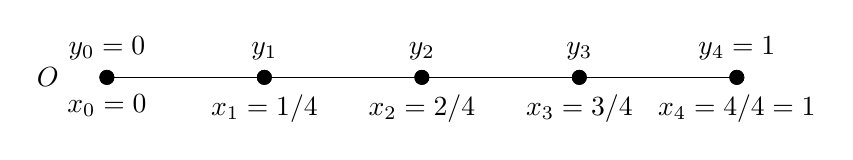
\begin{tikzpicture}
                \draw (0,0)--(8,0);
                \node at (-.75,0) {$O$};
                \node[circle,draw,fill=black,inner sep=0pt, minimum size=5pt,label=above:{$y_0=0$}] at (0,0) {};
                \node[circle,draw,fill=black,inner sep=0pt, minimum size=5pt,label=below:{$x_0=0$}] at (0,0) {};
                
                \node[circle,draw,fill=black,inner sep=0pt, minimum size=5pt,label=above:{$y_1$}] at (2,0) {};
                \node[circle,draw,fill=black,inner sep=0pt, minimum size=5pt,label=below:{$x_1=1/4$}] at (2,0) {};
                
                \node[circle,draw,fill=black,inner sep=0pt, minimum size=5pt,label=above:{$y_2$}] at (4,0) {};
                \node[circle,draw,fill=black,inner sep=0pt, minimum size=5pt,label=below:{$x_2=2/4$}] at (4,0) {};
                
                \node[circle,draw,fill=black,inner sep=0pt, minimum size=5pt,label=above:{$y_3$}] at (6,0) {};
                \node[circle,draw,fill=black,inner sep=0pt, minimum size=5pt,label=below:{$x_3=3/4$}] at (6,0) {};
                
                \node[circle,draw,fill=black,inner sep=0pt, minimum size=5pt,label=above:{$y_4=1$}] at (8,0) {};
                \node[circle,draw,fill=black,inner sep=0pt, minimum size=5pt,label=below:{$x_4=4/4=1$}] at (8,0) {};
                \end{tikzpicture}
        \end{center}
        \begin{ex}
            Consider the equation \(y''+y+1=0\) with the boundary conditions \(y(0)=0\), \(y(1)=0\).
        \end{ex}
\begin{soln}
    Here \(nh=1\). The differential equation is approximated as
    \[
        \frac{y_{i-1}-2y_i+y_{i+1}}{h^2}+y_i+1=0
    \]
    and this gives after simplification,
    \[
        y_{i-1}-(2-h^2)y_i+y_{i+1}=-h^2;\qquad i=1,2,3,\dots,n-1
    \]
    Choose \(h=1/4\) i.e., \(n=4\), we obtain the equations
    \begin{align*}
        &y_0-\frac{31}{16}y_1+y_2=-\frac{1}{16}\;\;\;
        \Rightarrow\;-\frac{31}{16}y_1+y+2=-\frac{1}{16}\quad[\because y_0=0]\\
        &y_1-\frac{31}{16}y_2+y_3=-\frac{1}{16}\\
        &y_2-\frac{31}{16}y_3+y_4=-\frac{1}{16}\;\;\;
        \Rightarrow\;y_2-\frac{31}{16}y_3=-\frac{1}{16}\quad[\because y_4=0]
    \end{align*}
    Solving the above system, we get,
    \[
        y_1=0.104677,\quad y_2=0.140312,\quad y_3=0.104677
    \]
    Hence \(y_2=y(0.5)=0.1140312\).
\end{soln}
\begin{ex}
    Consider the equation 
    \[
        y''=y;\qquad y(0)=0,\quad y(2)=3.627
    \]
    The finite difference approximation is written as
    \begin{align}
        &\frac{y_{i-1}-2y_i+y_{i+1}}{h^2}=y_i
        \label{eq:fde1}\\
        \Rightarrow\; & y_{i-1}-(2+h^2)y_i+y_{i+1}=0;\qquad i=1,2,3,\dots,n-1\notag
    \end{align}
    Taking \(h=0.5\), we have \(n=4\) and from \eqref{eq:fde1}
    \begin{align*}
        &4(y_0-2y_1+y_2)=y_1\\
        &4(y_1-2y_2+y_3)=y_2\\
        &4(y_2-2y_3+y_4)=y_3
    \end{align*}
    using \(y_0=0\) and \(y_4=3.627\), the above system becomes
    \[\systeme{
        -9y_1+4y_2=0,
        4y_1-9y_2+4y_3=0,
        4y_2-9y_3=-14.508
    }\]
    The solution of which is given in table below:
    \begin{table}
        \centering
        \begin{tabular}{cccc}
            \toprule
            \(x\)& Computed value of \(y\) & Exact value \(y=\sinh x\) & Error\\\midrule
            0.5 & 0.5262 & 0.5261 & 0.0051 \\
            1.0 & 1.1843 & 1.1752 & 0.0091 \\
            1.5 & 2.1382 & 2.1293 & 0.0089 \\ \bottomrule
        \end{tabular}
    \end{table}
\end{ex}
\begin{prob}[H.W.]
    Derive the finite difference approximation for nonlinear BVP.
\end{prob}
\begin{prob}[H.W.]
    Solve
    \begin{enumerate}
        \item \[y''=-\frac{2}{x}y'+\frac{2}{x^2}y+\frac{\sin(\log x)}{x^2};\quad 1\leq x\leq 2 \quad y(1)=1,\;y(2)=2\] by taking \(h=0.25\)
        \item \[y''=y'+2y+\cos x;\quad 0\leq x\leq \frac{\pi}{2} \quad y(0)=-0.3,\;y\left( \frac{\pi}{2} \right)=-0.1\] by using \(h=\frac{\pi}{4}\) and \(h=\frac{\pi}{6}\)
        \item \[y''=t+\left( 1-\frac{t}{5} \right)y; \quad y(1)=2,\;y\left(3\right)=-1\] by using \(h=0.5\)
    \end{enumerate}
    \begin{center}
        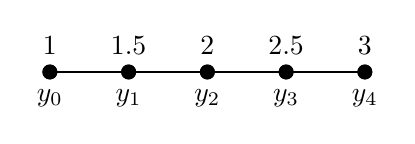
\begin{tikzpicture}
            \draw (0,0)--(4,0);
            \node[circle,draw,fill=black,inner sep=0pt, minimum size=5pt,label=above:{$1$}] at (0,0) {};
            \node[circle,draw,fill=black,inner sep=0pt, minimum size=5pt,label=below:{$y_0$}] at (0,0) {};
            
            \node[circle,draw,fill=black,inner sep=0pt, minimum size=5pt,label=above:{$1.5$}] at (1,0) {};
            \node[circle,draw,fill=black,inner sep=0pt, minimum size=5pt,label=below:{$y_1$}] at (1,0) {};
            
            \node[circle,draw,fill=black,inner sep=0pt, minimum size=5pt,label=above:{$2$}] at (2,0) {};
            \node[circle,draw,fill=black,inner sep=0pt, minimum size=5pt,label=below:{$y_2$}] at (2,0) {};
            
            \node[circle,draw,fill=black,inner sep=0pt, minimum size=5pt,label=above:{$2.5$}] at (3,0) {};
            \node[circle,draw,fill=black,inner sep=0pt, minimum size=5pt,label=below:{$y_3$}] at (3,0) {};
            
            \node[circle,draw,fill=black,inner sep=0pt, minimum size=5pt,label=above:{$3$}] at (4,0) {};
            \node[circle,draw,fill=black,inner sep=0pt, minimum size=5pt,label=below:{$y_4$}] at (4,0) {};
            \end{tikzpicture}
    \end{center}
    Ans: \(y_1=y(1.5)=0.552\), \(y_2=y(2.0)=-0.424\), \(y_3=y(2.5)=-0.964\). 
\end{prob}
\end{document}